\subsection{Diagrammi dei package}
Il seguente capitolo descrive le dipendenze intercorse fra i vari package\ped{G} del sistema Sequenziatore.

Il sistema Sequenziatore è composto da due macro package:
\begin{enumerate}
	\item sequenziatore.client: le componenti di questo package realizzano la parte front-end\ped{G} del sistema Sequenziatore 
	\item sequenziatore.server: le componenti di questo package realizzano la parte back-end\ped{G} del sistema Sequenziatore 
\end{enumerate}
\subsubsection{Diagrammi del package \client{}}

\begin{figure}[H] \centering 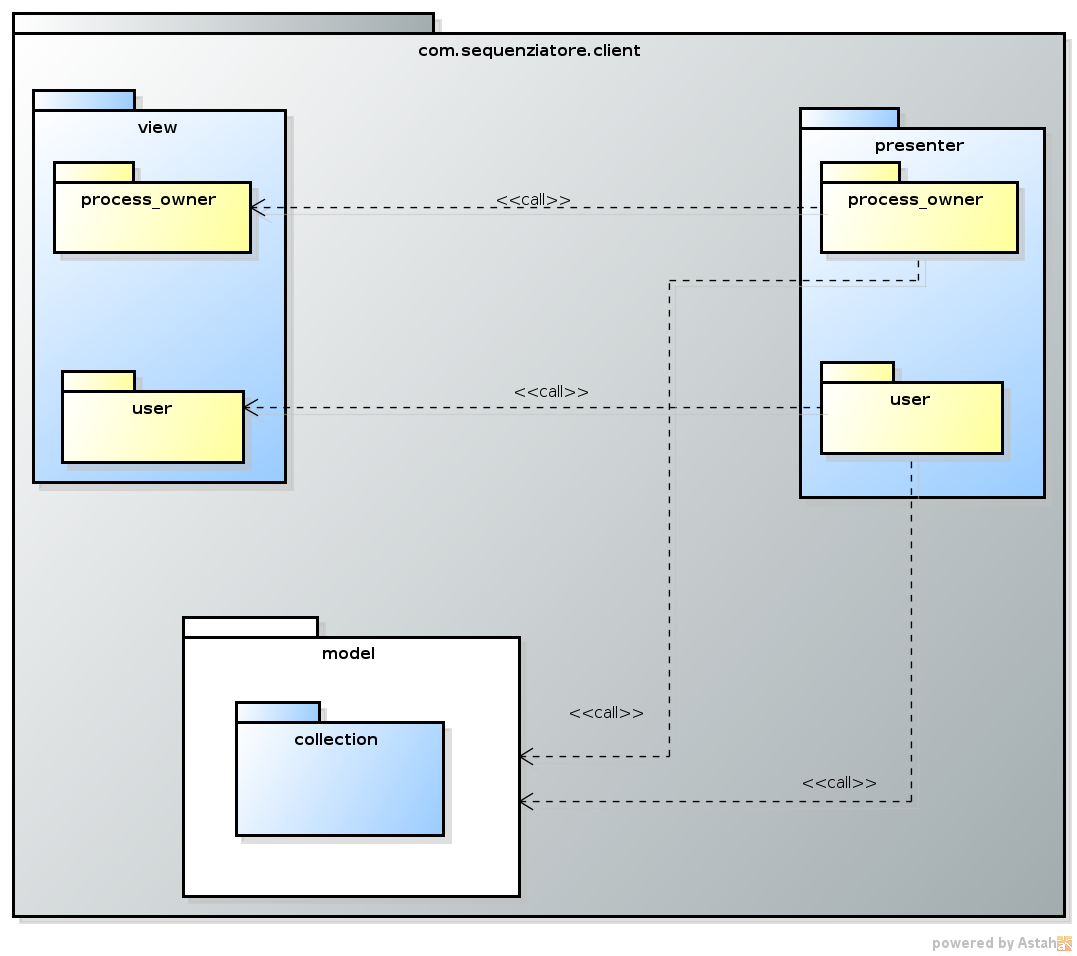
\includegraphics[width=%
\textwidth]
{./pack/Client.png} \caption{Diagramma package - \textit{\client{}}}
\end{figure}

Il package sequenziatore.client è composto dai seguenti package:
\begin{itemize}
	\item \view{};
	\item \logic{};
	\item \model{}.
\end{itemize}

Come è facilmente intuibile, la struttura del package \client{} si basa sulla struttura del design patter
architetturale Model View Presenter, scelto dal team Sirius per poter separare la logica di presentazione dei dati dalla logica di business.\\

\paragraph{Package \view{}}
Il package \view{} è composto da i seguenti package:
\begin{itemize}
	\item \viewAdmin{}: contiene le classi e interfacce necessarie a gestire 
l’interfaccia grafica e a generare gli eventi della parte grafica dell'utente process owner .
	\item \viewUser{}: contiene le classi e interfacce necessarie a gestire l’interfaccia
grafica e a generare gli eventi della parte grafica dell’utente.
\end{itemize}
\paragraph{Package \logic{}}
Il package \logic{} contiene tutte le classi e interfacce del Presenter della 
parte client\ped{G} del sistema Sequenziatore; ed è composto da i seguenti package:
\begin{itemize}
	\item \logicAdmin{}: contiene le classi che costituiscono la componente Presenter
per l’utente amministratore, il package \logicAdmin{} permette gestisce gli eventi generati dalle componenti del package \viewAdmin{} e 
aggiorna la parte grafica dell'utente process owner;
	\item \logicUser{}: contiene le classi che permettono la gestiscione degli gli eventi generati dalle componenti del package\ped{g}
\viewUser{} e l'aggiornamento della parte grafica per l'utente generico e autenticato.
\end{itemize}
\paragraph{Package \model{}}
Il package \model{} contiene tutte le classi della componente Model. Ogni classe del package \model{} possiede gli opportuni metodi per poter
comunicare col server e poter accedere, modificare e salvare in modo persistente questi ultimi.
Il package è contiene inoltre il package:
\begin{itemize}
	\item \collection{}: è composto da classi che implementano collezioni di classi del package \model{}.
\end{itemize} 


\subsubsection{Diagrammi del package \server{}}
I package che compongono il package \server{} sono:
\begin{itemize}
\end{itemize}

